\documentclass[11pt, oneside]{article}   	% use "amsart" instead of "article" for AMSLaTeX format


\usepackage{geometry}                		% See geometry.pdf to learn the layout options. There are lots.
\geometry{letterpaper}                   		% ... or a4paper or a5paper or ... 
%\geometry{landscape}                		% Activate for for rotated page geometry
%\usepackage[parfill]{parskip}    		% Activate to begin paragraphs with an empty line rather than an indent
\usepackage{graphicx}				% Use pdf, png, jpg, or eps§ with pdflatex; use eps in DVI mode
								% TeX will automatically convert eps --> pdf in pdflatex		
\usepackage{amssymb}
\usepackage{verbatim}
\usepackage{amsmath,amsthm,amsfonts,amssymb,amscd,hyperref}
\usepackage{framed}

\usepackage{graphicx,subfigure}
\usepackage{epsfig}
\usepackage{hyperref}
\usepackage{amsmath}
\usepackage{amssymb}
\usepackage{algorithm}
\usepackage{algorithmic}
\usepackage{url}
\usepackage{enumerate}
\usepackage{amsfonts}
\usepackage{boxedminipage}
\usepackage{xcolor}
 \usepackage{framed}  
\usepackage{rotating}
\usepackage{array}
\usepackage{multirow}
\usepackage{color}
\usepackage{tikz}
\usepackage{mathabx}
\usepackage{tabularx,ragged2e,booktabs,caption}
%\usepackage{enumitem}

\newtheorem{lemma}{Lemma}
\newtheorem{theorem}[lemma]{Theorem}
\newtheorem{corollary}[lemma]{Corollary}
\newtheorem{definition}[lemma]{Definition}
\newtheorem{proposition}[lemma]{Proposition}
\newtheorem{claim}[lemma]{Claim}
\newtheorem{question}{Question}
\newtheorem{remark}[lemma]{Remark}
\newtheorem{example}[lemma]{Example}
\newtheorem{exercise}{Exercise}
% * <plusel@gmail.com> 2018-03-21T21:05:07.197Z:
%
% > \newtheorem{lemma}{Lemma}
% > \newtheorem{theorem}[lemma]{Theorem}
% > \newtheorem{corollary}[lemma]{Corollary}
% > \newtheorem{definition}[lemma]{Definition}
% > \newtheorem{proposition}[lemma]{Proposition}
% > \newtheorem{claim}[lemma]{Claim}
% > \newtheorem{question}{Question}
% > \newtheorem{remark}[lemma]{Remark}
% > \newtheorem{example}[lemma]{Example}
% > \newtheorem{exercise}{Exercise}
%
% ^.
\newcommand{\E}{\mathbb{E}}

\usepackage[inline]{enumitem}


\title{{\large{Introduction to Machine Learning (67577)}}\\
\vphantom{}Recitation 1 \\
Recap Linear Algebra and Geometric Objects}

\date{March 16, 2016}

\begin{document}
\maketitle

\tableofcontents
\pagebreak




\section{Linear Transformation}

\begin{definition}[linear transformation]
Let $V$ and $W$ be two vector spaces over $\mathbb R$. A function $T:V\rightarrow W$ is called a linear transformation of $V$ into $W$, if the following two properties are true for all $u, v \in V$ and scalar $c\in \mathbb R$.
\begin{itemize}
\item $T(u+v) = T(u)+T(v)$. (additivity)
\item $T (cu) = cT (u)$. (scalar multiplication)
\end{itemize}
\end{definition}
properties (check it!) : $T(0)=0$, $T(-v)=-T(v)$, $T(u-v)=T(u)-T(v).$  \\

 If $V$  and $W$ are finite-dimensional , then any linear transformation can be represented by a matrix $A$. From now and on we will focus only on finite-dimensional spaces, and therefore won't distinguish between $T$ and its matrix representation $A$. \\

 
\begin{definition}[affine transformation]
An \textit{affine transformation} is a transformation of the form $T(x)=Ax+a.$
\end{definition}
 
  We will denote the \textit{Transpose} of such a linear transformation as $A^\top$.  \\
   $A^\top$ defines a linear transformation  $A^\top:W\to V$ .\\
  
  \begin{example}
  Here is a linear transformation from $\mathbb R^2$ to   $\mathbb R^3$ , and its transpose.
  \[A=\left( \begin{array}{ccc}
2 & 3 & 1\\
4 & 1  & -7 \end{array} \right) ~~\Rightarrow~~
  A^\top=\left( \begin{array}{ccc}
2 & 4  \\
3 & 1  \\
1 & -7\end{array} \right)\] 
 
 \end{example}
 
 What can you say about $(A^\top)^\top$?
~\\ 
  What happens when we multiply a matrix by a standard unit vector $A\hat{e_1}$ ?
\[
  \left( \begin{array}{ccc}
2 & 3 & 1\\
4 & 1  & -7 \end{array} \right) 
\left( \begin{array}{ccc}
1\\
0\\
0 \end{array} \right) =
\left( \begin{array}{ccc}
2\\
4 \end{array} \right) 
\]
  What about multiplying by an arbitrary vector $v$? 
  $$Av=A \left( a_1\hat{e_1}+a_2\hat{e_2}+a_3\hat{e_3}\right)=a_1A\hat{e_1}+a_2A\hat{e_2}+a_3A\hat{e_3}=a_1\cdot A_1+a_2\cdot A_2+a_3\cdot A_3$$
where $A_i$ is the $i$-th column of $A$. In other words, $Av$   is a linear combination of $A_i$ and the set of all possible $Av$ is actually all possible linear combinations of $A$'s columns! \\
~\\
 That leads us to define some properties of a linear transformation $A$:\\
\begin{itemize}
\item $im(A)=\{w\in W:w=Ax,x\in V\}$    \textit{(image / column space)}
\item $im(A^\top)=\{x\in V:x=A^\top w,w\in W\}$    \textit{(row space)}
\item $ker(A)=\{x\in V:Ax=0\}$  \textit{(The kernel)}
\end{itemize}

Note that by definition, $ker(A), row(A)\subseteq V$ and $im(A)\subseteq W$. Furthermore, you will prove it in the Targil an important fact:  each of the three is a vector subspace.

To know more about those three subspaces (and about a fourth subspace that we didn't mention here), watch the excellent MIT lecture \href{https://youtu.be/nHlE7EgJFds}{"The Four Fundamental Subspaces"} .
\begin{example}
Let's look at a very simple linear transformation from $\mathbb R^3$ to $\mathbb R$ : $A=\left( \begin{array}{ccc}
3,\
1,\
-2\end{array} \right) $
\begin{itemize}
\item $im(A)=\mathbb R$ 
\item $im(A^\top)$ is the line $(3\alpha ,\alpha ,-2\alpha )$  in $\mathbb R$.
\item $ker(A)$ is the set of all vectors orthogonal to $(3,1 ,-2)$ . That is \textbf{a hyperplane}. 
\end{itemize}
\end{example}
We will go back to the hyperplane later. meanwhile just remember that it is the kernel of linear transformation.\\

The column-space and the row-space magically have the same dimension. This allows us to define the \textit{rank} of a matrix:  $rank(A) = dim(im(A)) = dim(im(A^\top))$.\\
let $A$ be an $m\times n$ matrix. if $rank (A)<m,n$ then we say that $A$ is \textit{rank deficient}. Else, we say that $A$ is of \textit{full rank}.\\
A square matrix $A$ is said to be \textit{invertible}, if there exists another square matrix $B$ such that $AB=BA=I$.
Some equivalent conditions for invertibility of a square matrix:
\begin{itemize}
\item $A$ is full-rank
\item $det(A)\neq 0$
\item $im(A)=\mathbb R^n$ (i.e., the image is the whole space)
\item $ker(A)=\vec 0$
\end{itemize}
For a non-square matrix, the situation is a bit more delicate. There are a few definitions for a \emph{pseudo-inverse} matrix, and we will go back to it later.

\pagebreak
\section{Norm}


\begin{definition}[norm] 
A \emph{norm} is a function $||\cdot||:\mathbb{R}^m \rightarrow \mathbb{R}$ that satisfies the following three conditions for all $a \in \mathbb{R}$ and all $u, v \in \mathbb{R}^m$:
\begin{itemize}
\item $||av|| = |a|\cdot ||v||$ (Positive homogeneity)
\item $||u + v|| \leq ||u|| + ||v||$ (triangle inequality).
\item $||v|| = 0$ iff $v$ is the zero vector.
\end{itemize}
\end{definition}
Intuitively, a norm assigns each vector a length.
The above three properties are what we require from a function to conform to a reasonable notion of length.

\begin{exercise} Prove that the Euclidean norm is indeed a norm.  \end{exercise}

\begin{definition}[ball]
The \emph{unit ball} is:  $B = \{x| ||x|| \leq 1\}.$
\end{definition} 
\begin{figure}[h!]
  \centering
    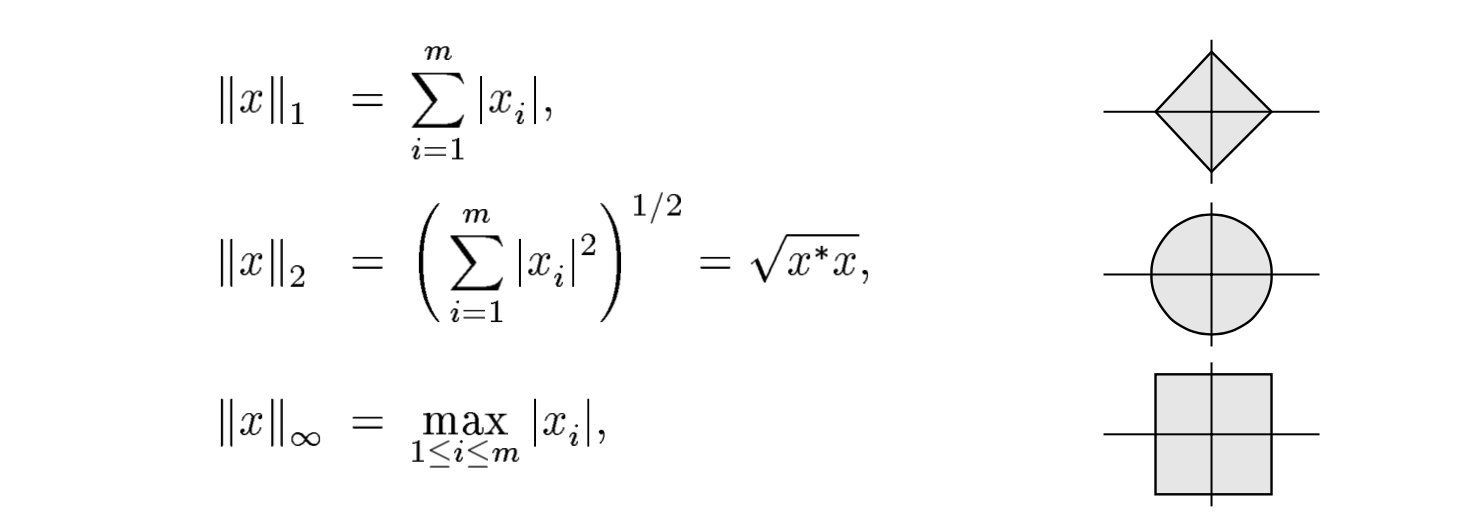
\includegraphics[scale=0.32]{norm.jpg}  
    \caption{A few famous norms, and the closed unit ball}
\end{figure}

Example: $||(1,0,-3,-2)||_1=|1|+|0|+|-3|+|-2|=6$

We will also use the $l_0$ ``norm"  which is equal to the number of the nonzero coordinates.

\begin{exercise}  Why is $l_0$ \emph{not} a norm?  \end{exercise}

\begin{exercise} Draw the unit ball of the  $l_0$ semi-norm. \end{exercise}

\pagebreak
\section{Inner product}


\begin{definition}[inner product]
Let  $x,y\in \mathbb{R}^d$ .
  $$\langle x,y\rangle=x^T\cdot y= \sum_{i=1}^n x_i\cdot y_i$$
 \end{definition}
 remark: vectors are \emph{column vectors}.\\
 Properties:
 \begin{itemize}
\item Symmetry: $\langle x,y\rangle=\langle y,x\rangle$
\item Linearity: for  $\alpha\in \mathbb R$ and  $x,y,z\in \mathbb R^d$ it holds that $\langle \alpha x+z,y\rangle=\alpha \langle x,y\rangle+\langle z,y\rangle$
\item Non-negativity : $\langle x,x\rangle\geq 0$  and $\langle x,x\rangle=0 \Leftrightarrow x=0$ 
 \end{itemize}
 Example: $\langle(1,1),(1,0)\rangle=1$. \\
 Example: $\langle(4,1),(-5,-2)\rangle=-22$. \\
 Example: $\langle(1,1),(1,1)\rangle=2$. \\
What's the connection between of the inner product $\langle x, x\rangle$ and length $||x||$?\\
We can define a length measure, the \emph{euclidean norm} $||x||=\sqrt{\langle x,x\rangle}$ (draw it for vector $(1,1)$)

\begin{exercise} Prove that  $\langle x,y\rangle=||x||\cdot||y||\cos\theta,$ where $\theta$ is the angle between $x$ and $y.$ \end{exercise}

Solution: Recall the Law of Cosines:  in a triangle with lengths $a,b,c$, then  $$c^2=a^2+b^2-2ab\cos\theta$$
Apply the cosine law for the triangle defined by $x$ and $y$. The third edge has a length of $x-y$, therefore:
$$ ||x-y||^2=||x||^2+||y||^2-2||x||\cdot||y||\cdot \cos \theta$$
On the other hand:
 $$ ||x-y||^2=\langle x-y,x-y\rangle=\langle x,x\rangle+\langle x,-y\rangle+\langle -y,x\rangle+\langle -y,-y\rangle=||x||^2+||y||^2-2\langle x,y\rangle$$
 Hence, $$||x||\cdot||y||\cdot \cos \theta = \langle x,y\rangle$$
 
Now, when we have a definition of angle though inner-product, we can define the projection of one vector onto the other.
\begin{definition}[vector projection]
A projection of a vector $v$ onto a vector $u$, is a vector $p$ of length $||v|| \cos \theta$ in the direction of $u$.
\end{definition}
Using the identity of $\cos\theta$:$$p=||v||\cos\theta\cdot \frac{u}{||u||}=||v||\frac{ \langle v,u\rangle}{||v||\cdot||u||}\cdot \frac{u}{||u||}=\frac{ \langle v,u\rangle }{||u||^2}\cdot u$$
\begin{figure}[h!]
  \centering
    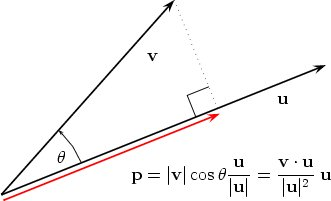
\includegraphics[scale=0.6]{v102x.jpg}  
   \caption{Vector projection}
\end{figure}
Example: vector projection of $(1,1)$ onto $(2,0)$ is equal to $\frac{1\cdot 2}{2^2}(2,0)=(1,0).$ \\
 
Notice, that for the special case: $\theta=90$ we get $\langle v,u\rangle=0$, in this case we say that the vectors $u,v$ are "orthogonals", or use the notation: $v\bot u$. If $u,v$ are also unit vectors we say that the vectors $u,v$ are "orthonormals".

\begin{definition}[orthogonal matrix]
An orthogonal matrix is a square matrix whose columns and rows are orthogonal unit vectors (i.e., orthonormal vectors)
\end{definition}

\begin{lemma}
Let $A\in M_{d\times d}(\mathbb{R})$ orthogonal matrix, we get:
$$AA^{T}=A^{T}A=I$$
\end{lemma}
 
 Using the inner-product we can talk about basic geometric objects in $\mathbb R^d$.
 Fix a vector $w\in \mathbb R^d$. What are the following objects?
 \begin{itemize}
 \item $\{x|\left<w,x\right>=0\}$
 \item $\{x|\left<w,x\right>\geq 0\}$
 \item $\{x-x_0|\left<w,x\right>\geq0\} = \{x|\left<w,x\right>\geq b\}$ (where $b=\left<w,x_0\right>$)
 \end{itemize}
\begin{definition}[Half-space]
 Fix $w\in \mathbb R^d$.  \emph{Half-space} is the set $\{x |\langle w,x\rangle \geq b\}$ and a \emph{hyperplane} is the set $\{x |\langle w,x\rangle = b\}.$
\end{definition}

\begin{figure}[h!]
  \centering
    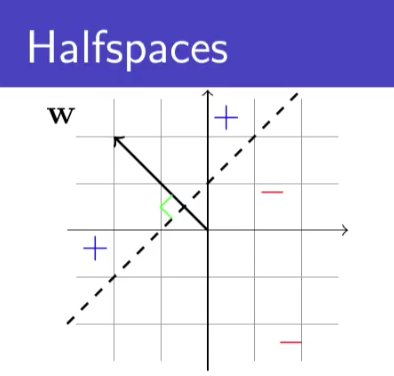
\includegraphics[scale=0.6]{halfspace.jpg}  
   %\caption{}
\end{figure}
 Note that we can also define half space by $sign(\langle w,x \rangle-b)\ge 0$.

\pagebreak
\section{Eigenvalue Decomposition (EVD)}

We first consider the case where $A$ is square and symmetric.
\begin{definition}[eigenvector and eigenvalue]
An eigenvector is a nonzero vector $v$ that satisfies the equation $Av=\lambda v$, where $A$ is a square matrix and $\lambda$ is the corresponding eigenvalue.
\end{definition}

\begin{theorem}[The spectral theorem for real symmetric matrices]
Every symmetric matrix $A\in M_{n\times n}$ can be expressed as $A=UDU^{T}$ where $U\in M_{n\times n}$ is orthogonal and $D\in M_{n\times n}$ is a diagonal matrix, i.e., the diagonal entries $D_{11},...,D_{nn}$ are the eigenvalues $D_{11}=\lambda_{1},D_{22}=\lambda_{2},\cdot\cdot\cdot,D_{nn}=\lambda_{n}$ and all other entries of D are zero.
\end{theorem}

This representation is extremely useful in many applications (e.g. calculating powers of $A$, $A^{3}=UDU^{T}\cdot UDU^{T}\cdot UDU^{T}=UD^{3}U^{T})$. However, it cannot be obtained when $m\neq d$, or even when $m=d$ but A is not symmetric. Nonetheless, as we will next see, we can obtain a slightly different representation which will also give us insight as to what A is doing.

\section{Singular Value Decomposition (SVD)}


\begin{theorem}["SVD Theorem"]
Every matrix $A\in$ $M_{m\times d}(\mathbb{R})$ admits a singular value decomposition of the form:
$$A=U\Sigma V^{\top}$$
where $U\in M_{m\times m}(\mathbb{R})$ and $V\in M_{d\times d}(\mathbb{R})$ are orthogonal matrices, and $\Sigma\in M_{m\times d}(\mathbb{R})$ is a diagonal matrix \bf{with none negative values}. 
\end{theorem}

Suppose that $rank\left(A\right)=r$. This means that the number of singular values is $r$, and notice that $r\le\min\left\{ d,m\right\}$ . When $m\le d$ then $A$ and $\Sigma$ are both wide matrices (they have more columns than rows), $A=U\Sigma V^{T}=$
\begin{eqnarray*}
\left(\begin{array}{ccccc}
\left(\begin{array}{c}
\\
\\
v_{1}\\
\\
\\
\end{array}\right) & ... & \left(\begin{array}{c}
\\
\\
v_{r}\\
\\
\\
\end{array}\right) & ... & \left(\begin{array}{c}
\\
\\
v_{m}\\
\\
\\
\end{array}\right)\end{array}\right)\left(\begin{array}{cccccc}
\sigma_{1} & \ldots & 0 & 0 & \ldots & 0\\
\vdots & \ddots & \vdots & \vdots & \ldots & \vdots\\
0 & \ldots & \sigma_{r} & 0 & \ldots & 0\\
0 & \ldots & 0 & 0 & \ldots & 0\\
0 & \ldots & 0 & 0 & \ddots & 0
\end{array}\right)\left(\begin{array}{c}
\left(\begin{array}{ccccc}
 & u_{1}^{\top} & \end{array}\right)\\
\vdots\\
\left(\begin{array}{ccccc}
 & u_{r}^{\top} & \end{array}\right)\\
\vdots\\
\left(\begin{array}{ccccc}
 &  u_{d}^{\top}& \end{array}\right)
\end{array}\right)
\end{eqnarray*}
The vectors $v_1...v_m$ are called left singular vectors, and the vectors $u_1...u_m$ are called right singular vectors.
\begin{exercise}
How will this look like when $m\ge$ d?
\end{exercise}

Since $\Sigma$ is diagonal, the non singular vectors, i.e. $u_{r+1},\dots,u_{m}$ and $v_{r+1},\dots,v_{d}$ are multiplied by 0. This means that we can reduce the representation to:
\begin{eqnarray*}
\left(\begin{array}{ccc}
\left(\begin{array}{c}
\\
\\
v_{1}\\
\\
\\
\end{array}\right) & ... & \left(\begin{array}{c}
\\
\\
v_{r}\\
\\
\\
\end{array}\right)\end{array}\right)\left(\begin{array}{ccc}
\sigma_{1} & \ldots & 0\\
\vdots & \ddots & \vdots\\
0 & \ldots & \sigma_{r}
\end{array}\right)\left(\begin{array}{c}
\left(\begin{array}{ccccc}
 & u_{1}^{\top} & \end{array}\right)\\
\vdots\\
\left(\begin{array}{ccccc}
 & u_{r}^{\top} & \end{array}\right)
\end{array}\right)
\end{eqnarray*}

Notice that now the matrices are of smaller dimensions – $\tilde{\Sigma}\in M_{r\times r}(\mathbb{R}), \tilde{U}\in M_{m\times r}(\mathbb{R})$ and $\tilde{V}\in M_{d\times r}(\mathbb{R})$.\\

The following lemma relates the SVD of A to the EVD of $AA^{\top}$ and $A^{\top}A$. In particular, it shows that the SVD of $A$ can be calculated in polynomial time in $m$ and $d$

\begin{lemma}
A matrix $A\in M_{m\times d}(\mathbb{R})$ has an SVD of the form $A=U\Sigma V^{\top}$ if and only if $AA^{\top}=U\Sigma\Sigma^{\top}U^{\top}$ is an EVD of $AA^{\top}$, and $A^{\top}A=V\Sigma^{\top}\Sigma V^{\top}$ is an EVD of $A^{\top}A$.
\end{lemma}

\begin{proof}
Left as an exercise.
\end{proof}

Notice that $\Sigma\Sigma^{T}$ and $\Sigma^{T}\Sigma$ are square diagonal matrices, with the same non-zero values on the diagonal. When A is square we get that $\Sigma\Sigma^{T}=\Sigma^{T}\Sigma=\Sigma^{2}$.

\section{Spectral Norm}

\begin{definition}[Isometric transformation]
Let $T:\mathbb{R}^{m}\rightarrow\mathbb{R}^{n}$ be linear transformation. We say that T is isometric if and only if: $||T(v)||=||v||$ for all $v\in \mathbb{R}^{m}$ 
\end{definition}

Linear isometries are distance-preserving maps, thus any linear isometrie can be interpreted as rotation or reflection of the axes (the basis of the vector space).

\begin{claim}
orthogonal matrix is isometric transformation.
\end{claim}

\begin{proof}
In the exercise.
\end{proof}

This observation enable as to give another interpretation to the SVD theorem:
Every linear transformation $A:\mathbb{R}^{n}\rightarrow\mathbb{R}^{m}$ (matrix $A\in$ $M_{m\times d}(\mathbb{R})$) admits a singular value decomposition of the form:
$$A=U\Sigma V^{\top}$$
which means that $T(w)$ is actually:
\begin{enumerate}
    \item rotation of w (multiply by orthogonal matrix V).
    \item stretch the rotated vector (multiply by diagonal matrix $\Sigma$).
    \item apply another rotation to the stretched vector(multiply by orthogonal matrix U).
\end{enumerate}  

\begin{figure}[h!]
  \centering
    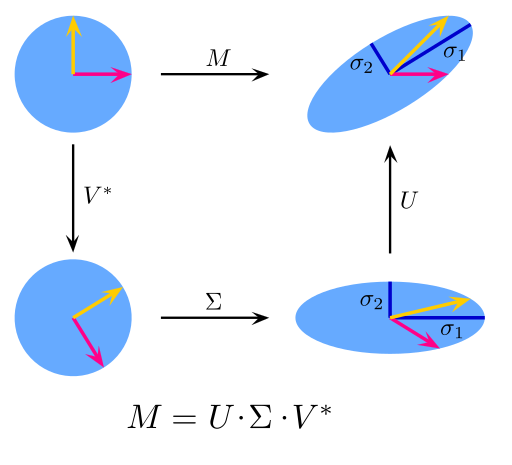
\includegraphics[scale=0.6]{svd_intuition.png}  
   \caption{SVD intuition}
\end{figure}

This insight lead as to the follow observation:
\begin{claim}
Let $U\Sigma V^{\top}$ be SVD decomposition of $A$, where $\Sigma=\left(\begin{array}{ccc}
\sigma_{1} &  & 0\\
 & \ddots\\
0 &  & \sigma_{k}
\end{array}\right)$ and $\sigma_{1}\ge...\ge\sigma_{k}$. than we get: $$\sigma_{1}=\max\frac{\left\Vert Ax\right\Vert }{\left\Vert x\right\Vert }$$
\end{claim}

\begin{proof}
First of all, since U is isometric:
\begin{align*}\max_{||x||_2 =1}||Ax||_2 & = \max_{||x||_2 =1}||U\Sigma V^Tx||_2 = \max_{||x||_2 =1}||\Sigma V^Tx||_2\end{align*}
Now let $y=V^{T}x$, By the same argument above $||y||_2 = ||V^Tx||_2 = ||x||_2 = 1$ so we have: $$\sup_{||x||_2 =1}||\Sigma V^Tx||_2 = \sup_{||y||_2 =1}||\Sigma y||_2$$
Since $\Sigma = \mbox{diag}(\sigma_1, \cdots, \sigma_n)$, where $\sigma_1$ is the largest singular value, the max for the above, $\sigma_1$, is attained when $y=(1,...,0)^{T}$.
\end{proof}

This size also known as the "spectral norm of A" (it is nice exercise to show that it is indeed norm)

\end{document}